\section{Detailkonzept} \label{sec:detailkonzept}

Das Konzept mit den Wasserliften ist am besten geeignet für unsere Anwendung. Es existieren bereits solche «Rohrkettenförderer», die jedoch Produkte hinaufbefördern. Wir nutzen dieses System um das Wasser nach unten zu befördern und dabei Energie zu gewinnen. Es werden insgesamt sechs Lifte benötigt. Fünf Lifte überwinden je 60.08\si{m} und der unterste Lift überwindet 80.24\si{m}. In der Abbildung \ref{fig:PrinzipGrobkonzept4} \nameref{fig:PrinzipGrobkonzept4} ist dies grafisch dargestellt.

\subsection{Elektronik}

\begin{figure}[H]
\centering
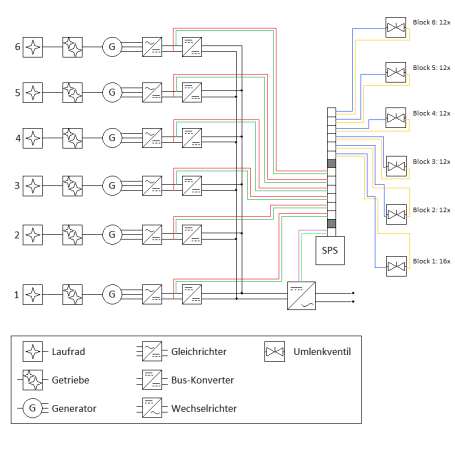
\includegraphics[width=\linewidth]{Skizze_GK4.png}
\caption{Prinzipschema}
\label{fig:Prinzipschema}
\end{figure}

\paragraph{Funktionsbeschreibung}

Die potentielle Energie des Abwassers wird über ein Laufrad in kinetische Energie umgewandelt. Mit einem Getriebe wird die vom Laufrad kommende Drehzahl dem Generator angepasst, dieser wandelt die kinetische Energie in elektrische um. Der Gleichrichter transformiert den 3 Phasen Drehstrom in einen 2 poligen Gleichstrom. Anschliessend wird durch ein DC-DC Konverter eine Rückkoppelung auf den Genreator verhindert. Weiter stellt der Konverter sicher, dass eine stabile Ausgangsspannung anliegt und das der DC-Bus galvanisch vom Generator und Wechselrichter getrennt ist. Die summierte Energie aller sechs Generatorenstränge wird über einen Wechselrichter ins Stromnetz eingespeist. Zur Überwachung und auch zur Ansteuerung der Umlenkventile im Wartungsfall wird eine SPS verwendet.

\paragraph{Generator}

%TODO Lars: Tagesgangkurve beschreiben und dadurch mindestleitung Generator (3kW) begründen: (Tagesenergie 191.1MJ)

\begin{figure}[H]
\centering
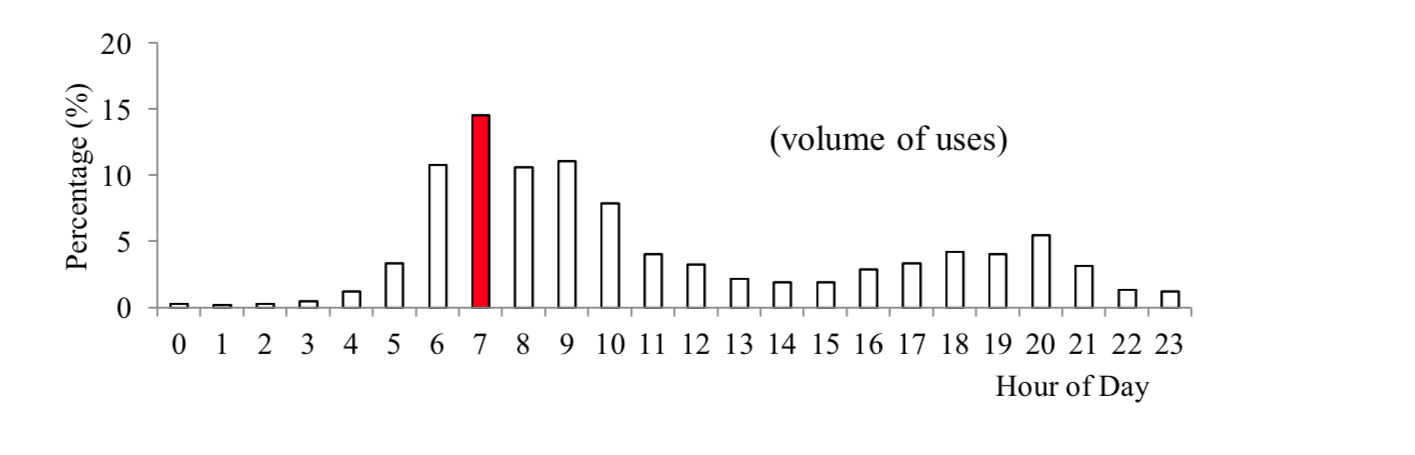
\includegraphics[width=\linewidth]{tagesGangKurve.png}
\caption{Typische Tagesgangkurve. \cite{peakWaterDemand}}
\label{fig:tagesGangKurve}
\end{figure}

%TODO Lars: Ausgesuchter Generator mit Kosten auflisten; Warum dieser Generator? Drehzahl beachten -> Zahnradsystem

\paragraph{Wechselrichter nach Generator}

%TODO Lars: Ausgesuchter Wechselrichter mit Kosten auflisten; Warum dieser Wechselrichter?

\paragraph{DC-DC Wandler}

%TODO Lars: Ausgesuchter DC-DC Wandler mit Kosten auflisten; Warum dieser DC-DC Wandler(Kein Strom darf zurückfliessen!)?

\paragraph{Wechselrichter für Netzeinspeisung} \label{par:WechselrichterNetz}

Damit die gewonnen Leistung in das Netz eingespiesen werden kann, muss der Wechselrichter folgende Eigenschaften aufweisen. 

\textbf{Leistung:}		9KW \newline
\textbf{Ausgang:}		3Phasen \newline
\textbf{Kosten:}		Die Kosten sollen möglichst gering gehalten werden. \newline

In der Förderungsanlage wird ein Asynchrongenerator verbaut. Die Firma Voltacon ist bekannt für ihre Hochleistungswechselrichter.

Das Model Hybrid Wechselrichter HSI10000 entspricht den gewünschten Anforderungen für unsere Förderungsanlage. Der Wechselrichter transformiert die 48VDC auf 230VAC mit einer Frequenz von 50\si{\hertz}. Das Gerät kann bis zu einer Leistung von 10KW erbringen. Mittels integrierten Displays kann die erbrachte Leistung zusätzlich abgelesen werden. 

Gemäss Datenblatt lassen sich Ströme bis 200A regeln. Der Wechselrichter hat einen netzunabhängigen Energiespeicher (Batterie-Backup). Um die Daten des Wechselrichters weiterzuleiten stehen verschieden Kommunikationsmittel zur verfügung. Die Informationen können über einen USB Port, RS-232 oder den SNMP (Simple Network Management Protocol) Überwachungssoftware für Echtzeitstatusanzeige und-steuerung übermittelt werden. Die kosten des Wechselrichters belaufen sich auf 3'401\si{Fr}.


\paragraph{Kontrollsystem}

Das Kontrollsystem steuert und überwacht die Anlage und ist wie folgt aufgebaut: Auf einem PC ist eine C\# Software installiert. Das Programm kommuniziert über ModbusTPC mit der SPS und kann die Anlage so steuern. Über eine GUI kann ein Benutzer einfach auf die Anlage zugreifen, steuern und Informationen ablesen. Das Programm hat zwei verschiedene Modi. Einen Manuellen-Modus und einen Betriebs-Modus. Im Manuellen-Modus kann der Betrieb der Anlage für Wartungsarbeiten angepasst werden. So können die Ventile einzeln oder blockweise geschaltet werden. Im Betriebs-Modus werden nur im Störungsfall die Ventile automatisch geschalten um die Sicherheit zu gewährleisten. Wenn möglich werden nur einzelne Blöcke deaktiviert damit die Anlage weiterhin Strom produzieren kann. In beiden Modi wird die Stromgewinnung überwacht. So wird angezeigt welcher Generator gerade Strom erzeugt. Der Wechselrichter, der unter Wechselrichter für Netzeinspeisung beschrieben ist, kann über einem USB-Port eine serielle Kommunikation mit dem PC aufbauen. Das Programm kann die Informationen der aktuellen Energiegewinnung über diese Schnittstelle auslesen, speichert diese in einem Log. File und gibt diese an die Benutzeroberfläche weiter. Die gesammelten Daten können im Programm ausgewertet und grafisch dargestellt werden. Für dieses Kontrollsystem werden folgende Komponente benötigt.

\begin{table}[H]
\begin{tabular}{lllll}
\textbf{Anzahl}&\textbf {Komponente}&\textbf{Bezeichnung}&\textbf{Stückpreis [\si{Fr}]}&\textbf{Gesamtpreis [\si{Fr}]}\\
\hline
1&Kontrollklemme&BK9050&200&200\\
20&Digitale Ausgangsklemme&KL1114&100&2000\\
20&Digitale Eingangsklemme&KL2134&100&2000\\
7& Analoge Eingangsklemme&KL2134&100&700\\
1&PC&Dell&1000&1000\\
\hline
\end{tabular}
\end{table}

Die Kosten für die Komponenten betragen 5900 \si{Fr}. Für die Entwicklung der Software werden 3 PM benötigt und kostet einmalig 48'000\si{Fr}. 

\newpage


\subsection{Mechanik}

\paragraph{Rohrkette}

In der Industrie werden Rohrkettenförderer für den Transport von Schuttgüter verwendet. In der Abbildung \ref{fig:Rohrkettenfoerderer} \nameref{fig:Rohrkettenfoerderer} ist der Innenaufbau eines solchen Rohrkettenförderers ersichtlich.

\begin{figure} [H]
	\centering
	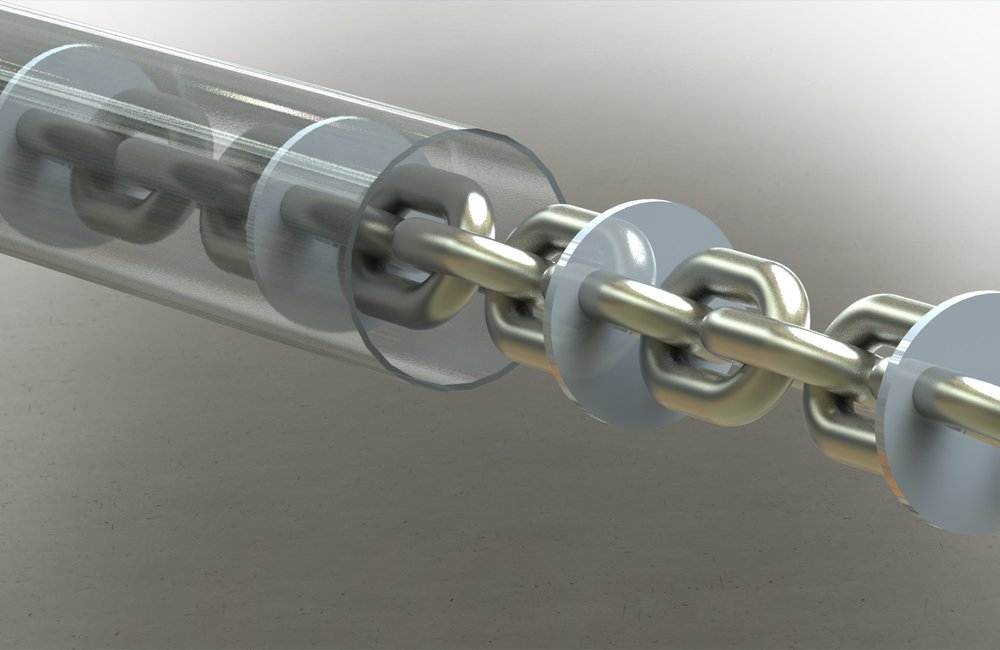
\includegraphics[width=6cm]{Rohrkettenfoerderer.jpg}
	\caption{Innenaufbau Rohrkettenförderer \cite{abconvey}}
	\label{fig:Rohrkettenfoerderer}
\end{figure}

Wir wollen keinen Schutt nach oben befördern, daher muss dieses System auf unsere Anforderungen angepasst werden. Diese Anforderungen sind, dass die verwendeten Materialien Robust gegenüber Korrasion sind, da das Abwasser aggressiv auf diese wirkt. Weiter müssen, um einen möglichst hohen Wirkungsgrad zu erreichen, die Platten mit möglichst kleinem Spielraum zur Ausserwand konstruiert werden, damit das Wasser nicht einfach auf der Seite herunterfliessen kann und gleichzeitig nicht eine zu grosse Reibung erzeugt wird. Die Drehachse, an dem der Generator angeschlossen wird ist ein Stösselkettenrad. Dieser ist in der Abbildung \ref{fig:stoesselkettenrad} \nameref{fig:stoesselkettenrad} zu sehen

\begin{figure} [H]
	\centering
	\includegraphics[width=6cm]{Stoesselkettenrad.jpg}
	\caption{Stösselkettenrad \cite{schrage}}
	\label{fig:stoesselkettenrad}
\end{figure}


Um diesen Wasserlift zu bauen beauftragen wir die Firma Schrage, ein führender Speziallist für Rohrketten, die in Deutschland zu Hause ist, beauftragt. Die Kosten belaufen sich für die 60.08\si{m} Höhendifferenz auf ca. 10'000\si{Fr} pro Lift und für die 80.24\si{m} Höhendifferenz auf ca. 13'000\si{Fr}. Insgesamt würde die Analage mit den Rohrketten, Rohr und Stösselkettenrad ca.63'000\si{Fr} kosten. \cite{schrage}

\newpage

\paragraph{Zahnradsytem}
%TODO Lars: Mindestdrehzahl dem Generator anpassen. Raddurchmesser für den Richtiungswechsel der rohrketten. Einen guten Wert annehmen

\paragraph{Umleitventil}

%TODO Roni: Ventile aussuchen die das Wasser entweder in die Falleitung oder in das rohrketten rohr leitet
% Genaues Ventil aussuchen. Anforderung 24V, Korrisionsbeständig

Da wir für Störungsfälle eine Fallleitung eingeplant haben, muss ein Umleitungsventil installiert werden. Das Model F7125 3-Way Butterfly Valve ist optimal für diese Bedingung geeignet. Das zugehörige Steuerungsmodel PRXUP-3-T kann von einer Spannung von zwischen 24V-230V angesteuert werden, somit können wir es im SPS System integrieren.

\textbf{Preis Bypass:  \si{Fr} \newline
 

\cite{F7125}
\subsection{Kosten}

%TODO Sonntag: Alle Kosten zusammentragen